\documentclass[11pt]{article}

\input{./preamble.tex}

%%
%% DOCUMENT START
%%

\begin{document}


\newcommand{\widesim}[2][1.5]{
  \mathrel{\overset{#2}{\scalebox{#1}[1]{$\sim$}}}
}

\pagestyle{fancyplain}
\lhead{}
\chead{}
\rhead{}
\lfoot{\hrule UQ: Homework 3}
\cfoot{\hrule \thepage}
\rfoot{\hrule Ryan Skinner}

\noindent
{\Large Homework 3}
\hfill
{\large Ryan Skinner}
\\[0.5ex]
{\large ASEN 6519: Uncertainty Quantification}
\hfill
{\large Due 2016/03/29}\\
\hrule
\vspace{6pt}

%%%%%%%%%%%%%%%%%%%%%%%%%%%%%%%%%%%%%%%%%%%%%%%%%
%%%%%%%%%%%%%%%%%%%%%%%%%%%%%%%%%%%%%%%%%%%%%%%%%
\section*{Problem 1} %%%%%%%%%%%%%%%%%%%%%%%%%%%%
%%%%%%%%%%%%%%%%%%%%%%%%%%%%%%%%%%%%%%%%%%%%%%%%%
%%%%%%%%%%%%%%%%%%%%%%%%%%%%%%%%%%%%%%%%%%%%%%%%%

Use the Smolyak formula
\begin{equation}
\mathc{A}(q,d) = \sum_{q-d+1 \le |\mb{L}| \le q} (-1)^{q-|\mb{L}|} \; \binom{d-1}{q-|\mb{L}|} \; \left( I^{(L_1)} \otimes \cdots \otimes I^{(L_d)} \right)
\label{eq:smolyak}
\end{equation}
to identify and plot the tensor-product of $d=1$ Clenshaw-Curtis (CC) Smolyak sparse grids from which the example grid $\mathc{A}(q=4,d=2)$ in the problem statement is constructed. Comment on the polynomial accuracy of the $d=2$ grid, referencing appropriate literature as needed.

\subsection*{Solution}

With $q=4$ and $d=2$, the bounds of the sum in \eqref{eq:smolyak} are $3 \le |\mb{L}| \le 4$. This admits only the following values of $\mb{L} = \{ L_1, L_2 \}$:
\begin{align*}
|\mb{L}| = 3: &\qquad \{ 0,3 \} \qquad \{ 1,2 \} \qquad \hphantom{\{ 2,2 \}} \qquad \{ 2,1 \} \qquad \{ 3,0 \} \\
|\mb{L}| = 4: &\qquad \{ 0,4 \} \qquad \{ 1,3 \} \qquad \{ 2,2 \} \qquad \{ 3,1 \} \qquad \{ 4,0 \}
\end{align*}
Abscissas of the 1-D CC grids are computed with \lstinline|spquad|, and the tensor-products resulting in the constituent 2-D grids are plotted in \figref{fig:prob1}.

According to Burkardt\footnote{\url{http://people.sc.fsu.edu/~jburkardt/presentations/sandia_2009.pdf}}, the Clenshaw-Curtis Smolyak formula of level $q$ is precise for all polynomials of degree $2q+1$ or less. Thus our grid with $q=4$ is 9\th-order accurate, a result which is independent of the dimension $d$ (though increasing $d$ does increase the number of collocation points required).

\begin{figure}[h]
\centering
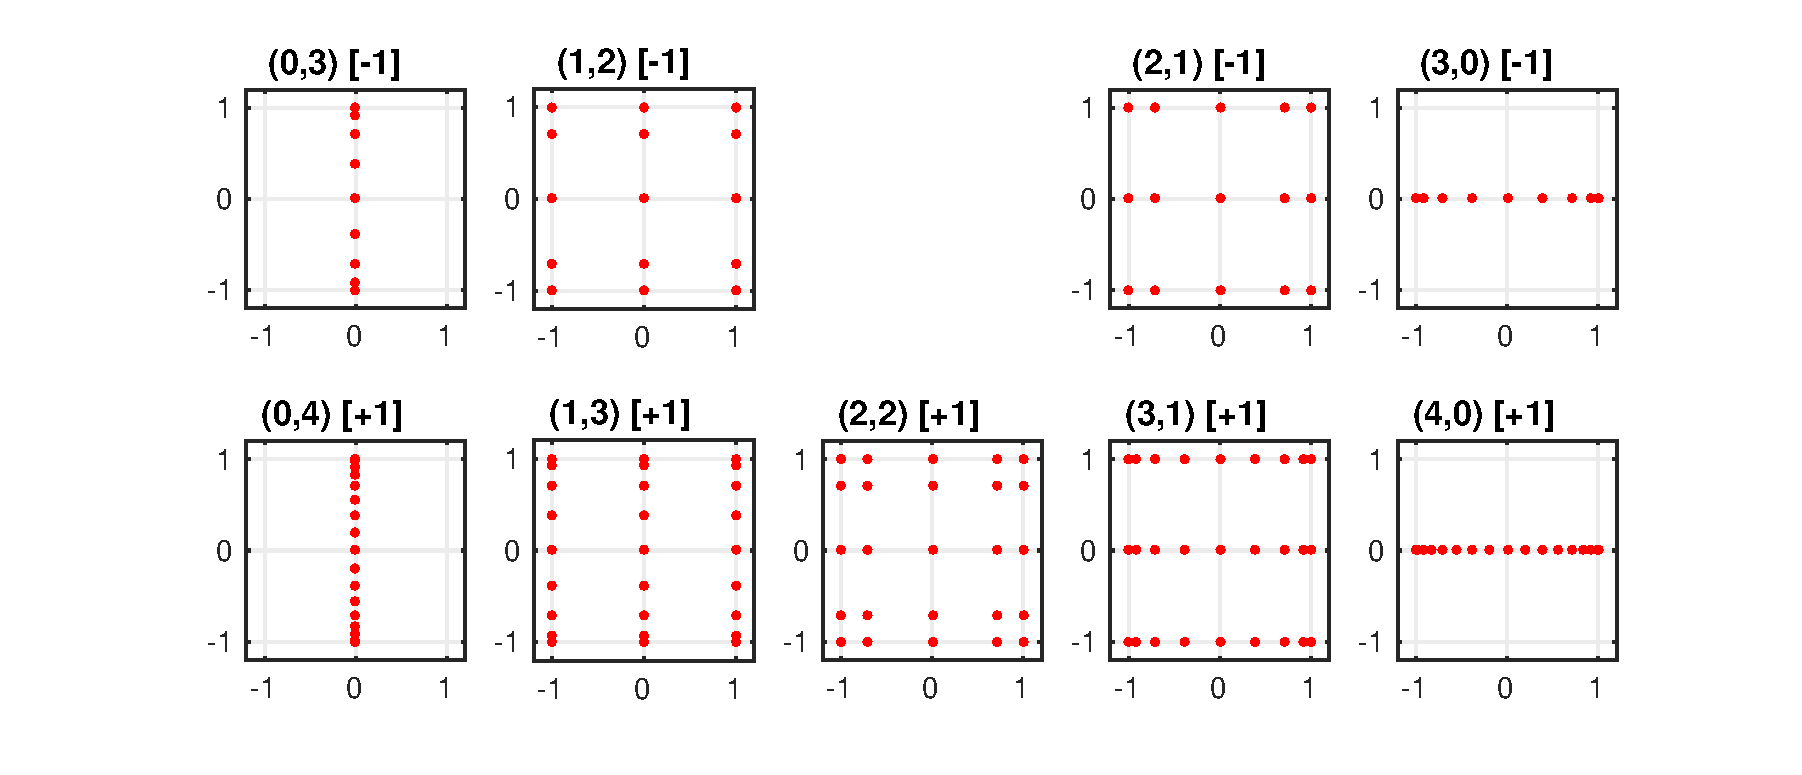
\includegraphics[width=0.9\textwidth, trim={1cm 0 1cm 0}]{prob1.eps}
\caption{Constituent grids that make up $\mathc{A}(4,2)$. Titles of sub-plots contain levels $L_1$ and $L_2$ in parentheses, and the value of $(-1)^{q-|\mb{L}|}$ in square brackets.}
\label{fig:prob1}
\end{figure}

%%%%%%%%%%%%%%%%%%%%%%%%%%%%%%%%%%%%%%%%%%%%%%%%%
%%%%%%%%%%%%%%%%%%%%%%%%%%%%%%%%%%%%%%%%%%%%%%%%%
\section*{Problem 2} %%%%%%%%%%%%%%%%%%%%%%%%%%%%
%%%%%%%%%%%%%%%%%%%%%%%%%%%%%%%%%%%%%%%%%%%%%%%%%
%%%%%%%%%%%%%%%%%%%%%%%%%%%%%%%%%%%%%%%%%%%%%%%%%

The thermal coefficient $K$ of a 1-D slab is defined on $\mathc{D} = (0,1)$ and is characterized by
\begin{equation}
K(x,\omega) = \overline{K} + \sigma \sum_{i=1}^d \sqrt{\lambda_i} \phi_i(x) y_i(\omega)
\end{equation}
where $\overline{K}=1$, $\sigma=0.1$, and $\{ \lambda_i, \phi_i(x) \}_{i=1}^d$ are eigen-pairs of the covariance kernel
\begin{equation}
C_{KK}(x_1,x_2) = \exp \left( \frac{- | x_1-x_2 | }{\ell} \right), \qquad (x1,x2) \in \mathc{D} \times \mathc{D}
\end{equation}

Moreover, $\{y_i\}$ are i.i.d. $U(-1,1)$. We would like to compute the statistics of the temperature field by solving the governing steady-state stochastic heat equation
\begin{equation}
\begin{aligned}
\pp{}{x} \left( K(x,\omega) \pp{u(x,\omega)}{x} \right) &= 1.0, \qquad x \in \mathc{D}, \\
u(0,\omega) &= 0, \\
u(1,\omega) &= 0,
\end{aligned}
\label{eq:pde}
\end{equation}

Setting $\ell = 2.0$, use the Homework \#1 code to compute the eigen-pairs $\{ \lambda_i, \phi_i(x) \}_{i=1}^d$ with $d=2$.

\begin{enumerate}

\item Compute $\xpect{u(x)}$ and $\var(u(x))$ of $u(x,\omega)$ using Latin Hypercube Sampling (LHS), with samples generated using your own code. Verify convergence of the mean and variance as you draw more samples.

\item Compute the same mean and variance using stochastic collocation with a tensor-product grid of the Clenshaw-Curtis rule. You can use the Matlab function \lstinline|spquad.m|, available on our course webpage, to obtain the abscissas and weights of the CC quadrature rule in dimension $d=1$. To obtain a reference solution for these comparisons, use $N=33$ quadrature points along each direction to compute the solution mean and variance. Verify convergence by increasing the number of quadrature points at $N = 1, 4, 16, 32$.

\item Compute the mean and variance using stochastic collocation of a Smolyak sparse grid with CC abscissas. Verify convergence in the manner discussed above.

\item On a single plot, compare the convergence of the estimates of the mean at $x=0.5$ based on standard Monte Carlo sampling, Latin Hypercube Sampling, tensor-product grid stochastic collocation (CC rule), and Smolyak sparse grid stochastic collocation (CC rule) as a function of the number of samples. Verify that the convergence rate of standard MC is $1/\sqrt{N}$. Repeat this comparison for the estimate of the variance at $x=0.5$.

\item Comment on the growth of the number of Smolyak abscissas and the feasibility of doing stochastic collocation when the correlation length is $\ell = 0.1$.

\end{enumerate}

\subsection*{Solution}

Convergence plots of the LHS, tensor-product CC, Smolyak sparse-grid CC, and MC sampling methods are show in Figures \ref{fig:prob2_lhs}, \ref{fig:prob2_dense}, \ref{fig:prob2_sparse}, and \ref{fig:prob2_mc}, respectively. All converge to nominally the same mean and variance as functions of position $x$. The number of collocation points used in each of these plots is shown in the legend.

Relative error in the mean and variance of temperature at $x = 0.5$ as a function of sampling points for each method is presented in \figref{fig:prob2_xp5}. The $N^{-1/2}$ convergence of the MC method's mean is confirmed visually by comparison to the line of slope $-1/2$ plotted on a log-log scale. A more rigorous confirmation of MC's convergence behavior in the mean could be carried out by computing the expectation of the sample mean's deviation from the true mean. This would require many experiments to be run for each value of $N$.

Though the Smolyak sparse-grid formula is better than tensor-product grids, it does not solve the curse of dimensionality. For large dimension $d$, the Clenshaw-Curtis Smolyak sparse grid uses $N \approx (2d)^p/p!$ collocation points to integrate a polynomial of total order $p$ exactly. This is $\bigo(d^c)$, which is a major improvement over tensor-product grids' $\bigo(c^d)$ scaling, where $c$ is a constant. Thus it still takes a large amount of computational effort to do stochastic collocation when the correlation length is $\ell = 0.1$, because it requires $d = 11$ eigenpairs to capture the stochastic behavior with below 10\% MSE, as shown in Homework \#1. A grid of $\mathc{A}(q=6,d=11)$ contains 280,017 collocation points, so this problem is still computationally tractable, but it is unclear exactly what levels $q$ are needed to accurately capture the mean and variance.

\begin{figure}[h]
\centering
\includegraphics[width=0.6\textwidth]{prob2lhs.eps}
\\[2ex]
\caption{Latin hypercube sampling (LHS) estimates of $\xpect{u(x)}$ and $\var(u(x))$ for a number $N$ of samples.}
\label{fig:prob2_lhs}
\end{figure}

\begin{figure}[h]
\centering
\includegraphics[width=0.6\textwidth]{prob2ccdense.eps}
\\[2ex]
\caption{Dense CC tensor-product estimates of $\xpect{u(x)}$ and $\var(u(x))$ for a number $N$ of samples.}
\label{fig:prob2_dense}
\end{figure}

\begin{figure}[h]
\centering
\includegraphics[width=0.6\textwidth]{prob2ccsparse.eps}
\\[2ex]
\caption{CC Smolyak sparse-grid estimates of $\xpect{u(x)}$ and $\var(u(x))$ for a number $N$ of samples.}
\label{fig:prob2_sparse}
\end{figure}

\begin{figure}[h]
\centering
\includegraphics[width=0.6\textwidth]{prob2mc.eps}
\\[2ex]
\caption{Monte Carlo estimates of $\xpect{u(x)}$ and $\var(u(x))$ for a number $N$ of samples.}
\label{fig:prob2_mc}
\end{figure}

\begin{figure}[h]
\centering
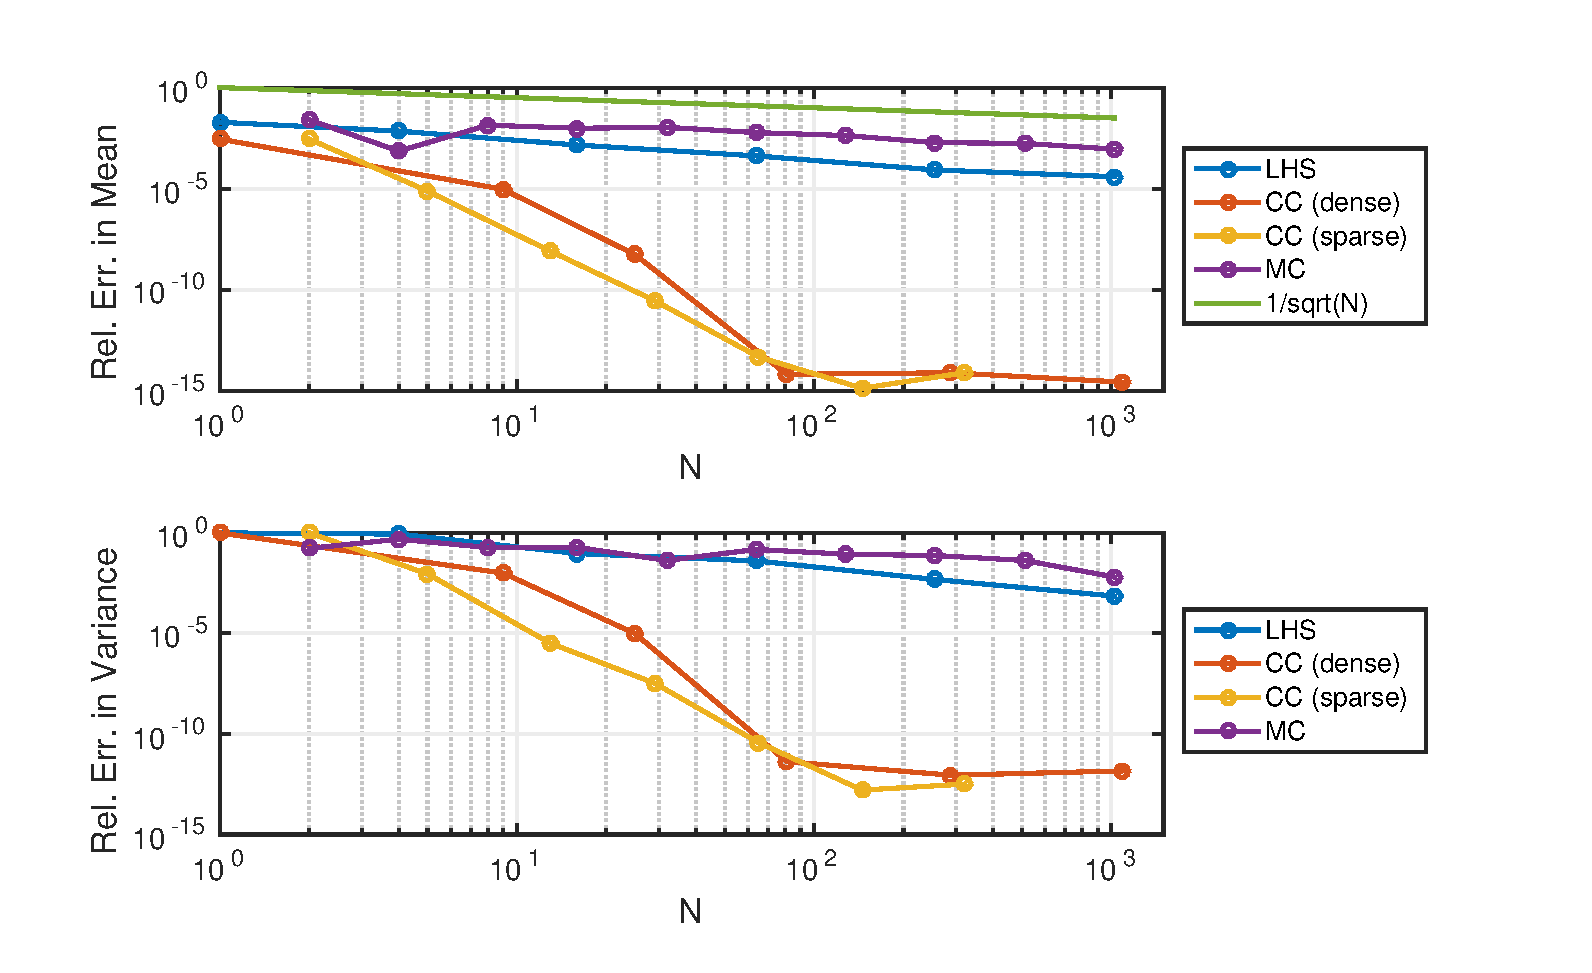
\includegraphics[width=\textwidth]{prob2xp5.eps}
\\[2ex]
\caption{Relative error in the mean and variance of different sampling techniques as a function of number $N$ of sampling points. Monte Carlo is seen to converge at a rate of approximately $1/\sqrt{N}$ in the mean, based on the slope of (MC) and (1/sqrt(N)). Reference ``truth'' values of the mean and variance are obtained with sparse CC sampling using 705 points in 2-D.}
\label{fig:prob2_xp5}
\end{figure}

%%
%% DOCUMENT END
%%
\end{document}
